\documentclass[tikz,border=6pt]{standalone}
\usepackage{amsmath}
\usetikzlibrary{arrows.meta}

\newcommand{\Kh}{\widehat K}
\newcommand{\Kt}{\widetilde K}
\newcommand{\hKot}{h_{K,1}}
\newcommand{\hKtt}{h_{K,2}}
\newcommand{\xt}{\widetilde x}

\begin{document}
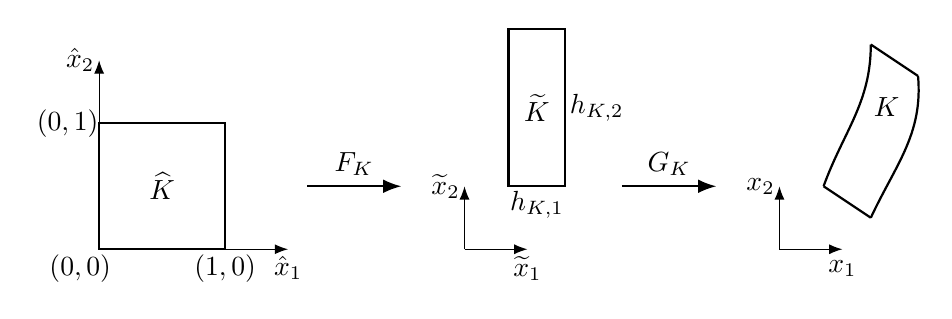
\begin{tikzpicture}[scale=.8,>=Latex]
  % Square
  \draw[thick] (0,0) rectangle (2,2);
  \node at (1,2.2) {};
  \node at (1,-0.2) {};
  \node[rotate=90] at (-0.4,1) {};
  \node[rotate=90] at (2.4,1) {};

  \draw[->] (0,0) -- (3,0);
  \draw[->] (0,0) -- (0,3);

  \node at (-0.3,3) {$\hat{x}_2$};
  \node at (3,-0.3) {$\hat{x}_1$};
  \node at (1,1) {$\Kh$};
  \node at (-0.3,-0.3) {$(0,0)$};
  \node at (2,-0.3) {$(1,0)$};
  \node at (-0.5,2) {$(0,1)$};

  % rectangle
  \draw[->, thick] (3.3,1) -- (4.8,1) node[midway, above] {$F_K$};
  \draw[thick] (6.5,1) rectangle (7.4,3.5);
  \node at (6.95,2.25) {$\Kt$};
  \node at (6.95,1-0.3) {$\hKot$};
  \node at (7.9,2.25) {$\hKtt$};
  \draw[->] (5.8,0) -- (5.8,1);
  \draw[->] (5.8,0) -- (6.8,0);
  \node at (5.8-0.3,1) {$\xt_2$};
  \node at (6.8,0-0.3) {$\xt_1$};

  % bent rectangle
  \draw[->, thick] (8.3,1) -- (9.8,1) node[midway, above] {$G_K$};
  \draw[thick]    (11.5,1) -- (12.25,0.5);
  \draw[thick]    (12.25,0.5) to[out=65,in=-85] (13,2.75);
  \draw[thick]    (13,2.75) -- (12.25,3.25);
  \draw[thick]    (12.25,3.25)  to[out=-90,in=70] (11.5,1);
  \draw[->] (10.8,0) -- (10.8,1);
  \draw[->] (10.8,0) -- (11.8,0);
  \node at (12.5,2.25) {$K$};
  \node at (10.8-0.3,1) {$x_2$};
  \node at (11.8,0-0.3) {$x_1$};
\end{tikzpicture}
\end{document}
